\documentclass[11pt]{article}
\usepackage{enumerate}
\usepackage{fullpage}
\usepackage{fancyhdr}
\usepackage{amsmath, amsfonts, amsthm, amssymb}
\usepackage{color}
\usepackage[]{graphicx}

\setlength{\parindent}{0pt}
\setlength{\parskip}{5pt plus 1pt}
\pagestyle{empty}

\def\indented#1{\list{}{}\item[]}
\let\indented=\endlist

\newcounter{questionCounter}
\newcounter{partCounter}[questionCounter]
\newenvironment{question}[2][\arabic{questionCounter}]{%
    \setcounter{partCounter}{0}%
    \vspace{.25in} \hrule \vspace{0.5em}%
        \noindent{\bf #2}%
    \vspace{0.8em} \hrule \vspace{.10in}%
    \addtocounter{questionCounter}{1}%
}{}
\renewenvironment{part}[1][\alph{partCounter}]{%
    \addtocounter{partCounter}{1}%
    \vspace{.10in}%
    \begin{indented}%
       {\bf (#1)} %
}{\end{indented}}

%%%%%%%%%%%%%%%%%%%%%%%HEADER%%%%%%%%%%%%%%%%%%%%%%%%%%%%%%
\newcommand{\myname}{Shashank Singh}
\newcommand{\myandrew}{sss1@andrew.cmu.edu}
\newcommand{\myclass}{86-595 Neural Data Analysis}
\newcommand{\myhwnum}{4}
\newcommand{\duedate}{Thursday, November 15, 2012}
%%%%%%%%%%%%%%%%%%%%%%%%%%%%%%%%%%%%%%%%%%%%%%%%%%%%%%%%%%%

%%%%%%%%%%%%%%%%%%%%CONTENT MACROS%%%%%%%%%%%%%%%%%%%%%%%%%
\newcommand{\ans}[1]{\mbox{\fbox{$\displaystyle #1$}}} % box around an answer in math mode
\renewcommand{\qed}{\quad $\blacksquare$} % black QED square
\newcommand{\mqed}{\quad \blacksquare} % black QED square for use in math mode
\newcommand{\inv}{^{-1}} % inverse
\newcommand{\blambda}{\boldsymbol{\lambda}}
\newcommand{\br}{\mathbf{r}}
\newcommand{\bx}{\mathbf{x}}
\newcommand{\by}{\mathbf{y}}
\newcommand{\bff}{\mathbf{f}}
\newcommand{\bzero}{\mathbf{0}}
\newcommand{\N}{\mathbb{N}} % natural numbers
\newcommand{\Q}{\mathbb{Q}} % rational numbers
\newcommand{\R}{\mathbb{R}} % real numbers
\newcommand{\E}[1]{\mathsf{E}\left[#1\right]} % expected value
\newcommand{\Var}[1]{\mathsf{Var}\left[#1\right]} % variance
\newcommand{\Poisson}[1]{\operatorname{Poisson}\left(#1\right)} % Poisson distribution
\newcommand{\Exp}[1]{\operatorname{Exp}\left(#1\right)} % Exponential distribution
\newcommand{\U}[2]{\operatorname{U}\left(#1,#2\right)} % Uniform distribution
\newcommand{\Bern}[1]{\operatorname{Bernoulli}\left( #1 \right)} % Bernoulli distribution
\newcommand{\pr}[1]{\mathsf{P}\left( #1 \right)} % probability of event #1
\newcommand{\giv}{\, | \,} % \pr{A \giv B} is the probability of A given B
\newcommand{\argmax}{\operatornamewithlimits{argmax}}
\newcommand{\argmin}{\operatornamewithlimits{argmin}}
%%%%%%%%%%%%%%%%%%%%%%%%%%%%%%%%%%%%%%%%%%%%%%%%%%%%%%%%%%%

\begin{document}
\thispagestyle{plain}

{\Large Homework \myhwnum} \\
\myclass \\
Name: \myname \\
Email: \myandrew \\
Due: \duedate \\
\begin{question}{Problem 1}
\begin{enumerate}[a.]
%TODO
\item Since we have no prior on signal probabilities and the utilities of
reporting signal and noise are uniform, we report a signal whenever the
likelihood ratio $\ell_{sn}$ of signal to noise is greater than $1$. Thus,
since the spike rate $r$ is distributed Poisson, we report a signal whenever
\begin{align*}
1
   < \ell_{sn}(r)
 & = \frac{\pr{r \giv s}}{\pr{r \giv n}}
   = \frac{\frac{30^r}{r!}e^{-30}}{\frac{20^r}{r!}e^{-20}} \\
 & = \left( \frac32 \right)^r e^{-10},
\end{align*}
which is the case precisely when
\fbox{$r > \log_{3/2}(e^{10}) \approx 24.7$.}

%TODO
\item Since we now have a prior on signal probabilities and the utilities of
reporting signal and noise are uniform, we report a signal whenever the
likelihood ratio $\ell_{sn}$ of signal to noise is greater than the ratio
$\frac{\pr{n}}{\pr{s}} = 4$ of the priors. Thus, following the
derivation in part (a),
\[4 < \left( \frac32 \right)^r e^{-10},\]
which is the case precisely when
\fbox{$r > \log_{3/2}(4e^{10}) \approx 28.1$.}

%TODO
\item Since we now have a prior on signal probabilities as well as nonuniform
utilities of reporting signal and noise, we report a signal whenever the
likelihood ratio $\ell_{sn}$ of signal to noise is greater than the ratio
$\frac{-U_{Sn}\pr{n}}{U_{Ss}\pr{s}} = 20$ of the priors and utilities, where
$U_{Ss} = 1$ is the utility of a true positive and $U_{Sn} = -5$ is the
utility of a false positive (we leave out the utilities of a true negative and
of a false negative, since they are $0$). Thus, following the derivation in
part (a),
\[20 < \left( \frac32 \right)^r e^{-10},\]
which is the case precisely when
\fbox{$r > \log_{3/2}(20e^{10}) \approx 32.1$.}

\end{enumerate}
\end{question}

\newpage
\begin{question}{Problem 2}
\begin{enumerate}[a.]
\item See Figure~\ref{fig:2.a}, which was generated by the following code:
\begin{figure}[h]
\begin{center}
\includegraphics[width=0.5\textwidth]{2.a.eps}
\end{center}
\caption{Choice accuracy over stimulus coherence. $\alpha, \beta$ were
estimated as $0.1, 1$, respectively.}
\label{fig:2.a}
\end{figure}
\begin{verbatim}
>> guesses = squeeze(MTdata(:,3,:));
>> correct = mean(guesses,1);
>> params = nlinfit(coherence, correct, @psychometric_curve, [0.1, 1]);
>> chance(1:65) = 0.5;
>> plot(0:0.01:0.64, chance, '--', 'Color','red');
>> plot(0:0.01:0.64, psychometric_curve(params, 0:0.01:0.64));
>> scatter(coherence, correct, 'filled');
\end{verbatim}

\item See Figure~\ref{fig:2.b}, which was generated by the following code:
\begin{figure}[h]
\begin{center}
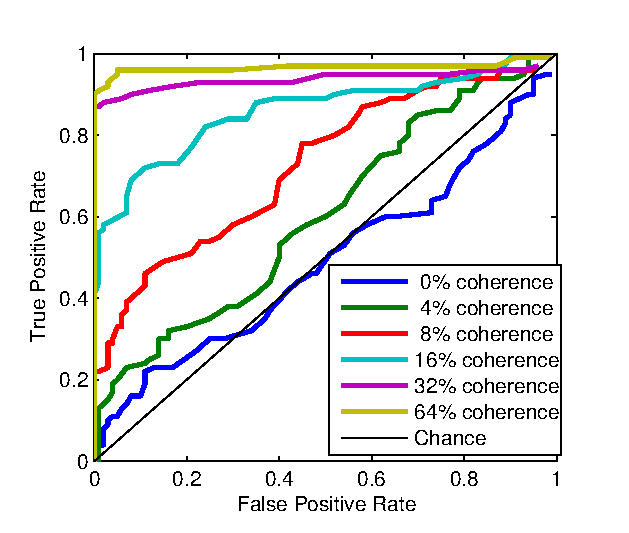
\includegraphics[width=0.5\textwidth]{2.b.eps}
\end{center}
\caption{ROC curves for neurons at each stimulus coherence.}
\label{fig:2.b}
\end{figure}
\begin{verbatim}
>> neurons = MTdata(:,1:2,:);
>> for i=1:100, roc(i,1:2,1:6) = mean(neurons > criterion(i)); end
>> for i=1:6, plot(squeeze(roc(:,1,i)), squeeze(roc(:,2,i)), 'Linewidth',2); hold all; end
>> plot(0:0.01:1,0:0.01:1,'color','black');
\end{verbatim}


\item Didn't have time to do this.

\item Didn't have time to do this.

\end{enumerate}
\end{question}
\end{document}
